\documentclass{beamer}

%
% Choose how your presentation looks.
%
% For more themes, color themes and font themes, see:
% http://deic.uab.es/~iblanes/beamer_gallery/index_by_theme.html
%
\mode<presentation>
{
  \usetheme{default}      % or try Darmstadt, Madrid, Warsaw, ...
  \usecolortheme{default} % or try albatross, beaver, crane, ...
  \usefonttheme{default}  % or try serif, structurebold, ...
  \setbeamertemplate{navigation symbols}{}
  \setbeamertemplate{caption}[numbered]
  \setbeamertemplate{footline}[page number]
  \setbeamercolor{frametitle}{fg=white}
  \setbeamercolor{footline}{fg=black}
} 

\usepackage[english]{babel}
\usepackage[utf8x]{inputenc}
\usepackage{tikz}
\usepackage{listings}
\usepackage{courier}

\xdefinecolor{darkblue}{rgb}{0.1,0.1,0.7}
\xdefinecolor{dianablue}{rgb}{0.18,0.24,0.31}
\definecolor{commentgreen}{rgb}{0,0.6,0}
\definecolor{stringmauve}{rgb}{0.58,0,0.82}

\lstset{ %
  backgroundcolor=\color{white},      % choose the background color
  basicstyle=\ttfamily\scriptsize,         % size of fonts used for the code
  breaklines=true,                    % automatic line breaking only at whitespace
  captionpos=b,                       % sets the caption-position to bottom
  commentstyle=\color{commentgreen},  % comment style
  escapeinside={\%*}{*)},             % if you want to add LaTeX within your code
  keywordstyle=\color{blue},          % keyword style
  stringstyle=\color{stringmauve},    % string literal style
  showstringspaces=false,
  showlines=true
}

\lstdefinelanguage{scala}{
  morekeywords={abstract,case,catch,class,def,%
    do,else,extends,false,final,finally,%
    for,if,implicit,import,match,mixin,%
    new,null,object,override,package,%
    private,protected,requires,return,sealed,%
    super,this,throw,trait,true,try,%
    type,val,var,while,with,yield},
  otherkeywords={=>,<-,<\%,<:,>:,\#,@},
  sensitive=true,
  morecomment=[l]{//},
  morecomment=[n]{/*}{*/},
  morestring=[b]",
  morestring=[b]',
  morestring=[b]"""
}

\title[2016-09-02-histogrammar-cuda]{Plotting data on GPUs}
\author{Jim Pivarski}
\institute{Princeton -- DIANA}
\date{September 2, 2016}

\begin{document}

\logo{\pgfputat{\pgfxy(0.11, 8)}{\pgfbox[right,base]{\tikz{\filldraw[fill=dianablue, draw=none] (0 cm, 0 cm) rectangle (50 cm, 1 cm);}}}\pgfputat{\pgfxy(0.11, -0.6)}{\pgfbox[right,base]{\tikz{\filldraw[fill=dianablue, draw=none] (0 cm, 0 cm) rectangle (50 cm, 1 cm);}
\includegraphics[height=0.99 cm]{diana-hep-logo.png}\tikz{\filldraw[fill=dianablue, draw=none] (0 cm, 0 cm) rectangle (4.9 cm, 1 cm);}}}}

\begin{frame}
  \titlepage
\end{frame}

\logo{\pgfputat{\pgfxy(0.11, 8)}{\pgfbox[right,base]{\tikz{\filldraw[fill=dianablue, draw=none] (0 cm, 0 cm) rectangle (50 cm, 1 cm);}
\includegraphics[height=1 cm]{diana-hep-logo.png}}}}

% Uncomment these lines for an automatically generated outline.
%\begin{frame}{Outline}
%  \tableofcontents
%\end{frame}

\begin{frame}{Motivated by a different problem}

I've been helping Oliver Gutsche, Matteo Cremonesi, Cristina Su\'arez port their dark matter search from C++ to Apache Spark.

\begin{center}

\includegraphics[width=0.8\linewidth]{spark.png}
\end{center}
\end{frame}

\begin{frame}{Motivated by a different problem}

\begin{block}{Histogramming in Spark}
\end{block}

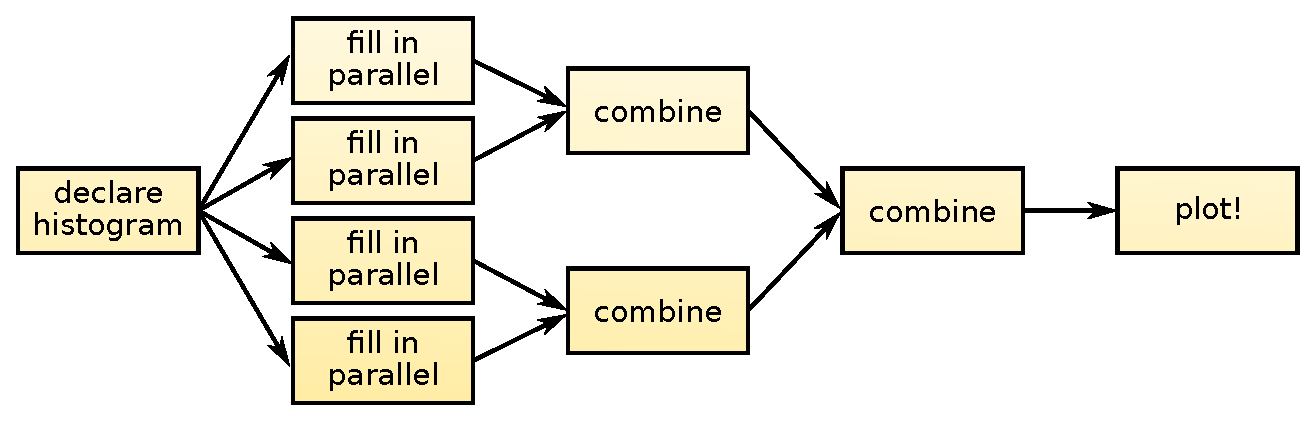
\includegraphics[width=\linewidth]{parallelization.pdf}

\vspace{-1 cm}
\[ \underbrace{\mbox{\hspace{1.5 cm}}}_{\mbox{head node}} \hspace{0.25 cm} \underbrace{\mbox{\hspace{6.5 cm}}}_{\mbox{executor nodes}} \hspace{0.5 cm} \underbrace{\mbox{\hspace{1.5 cm}}}_{\mbox{head node}} \]

\end{frame}

\begin{frame}{Motivated by a different problem}

\begin{block}{Histogramming on the GPU}
\end{block}

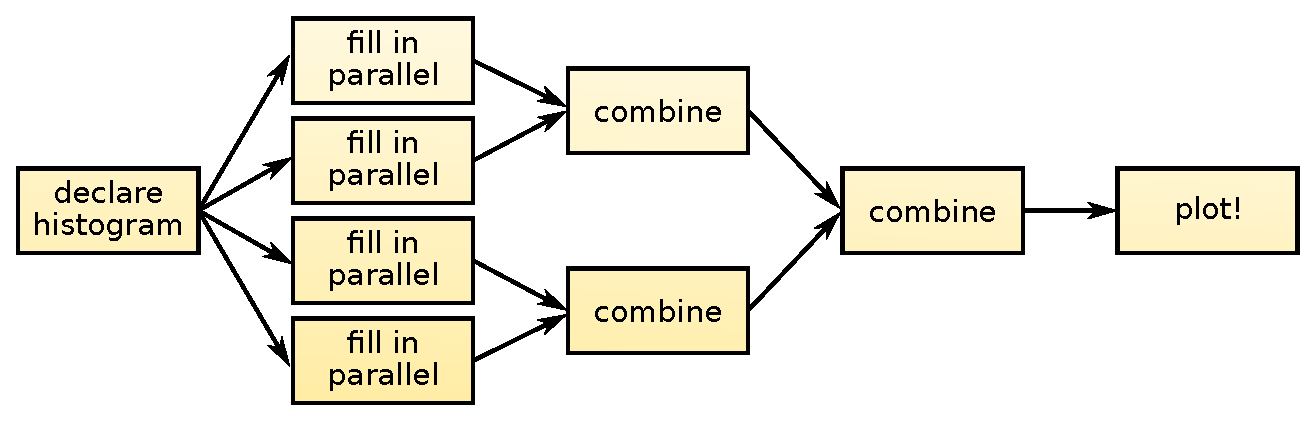
\includegraphics[width=\linewidth]{parallelization.pdf}

\vspace{-1 cm}
\[ \underbrace{\mbox{\hspace{1.5 cm}}}_{\mbox{host}} \hspace{0.25 cm} \underbrace{\mbox{\hspace{6.5 cm}}}_{\mbox{device}} \hspace{0.5 cm} \underbrace{\mbox{\hspace{1.5 cm}}}_{\mbox{host}} \]

\end{frame}

\begin{frame}{Motivated by a different problem}

\begin{block}{Histogramming in ROOT's PROOF system}
\end{block}

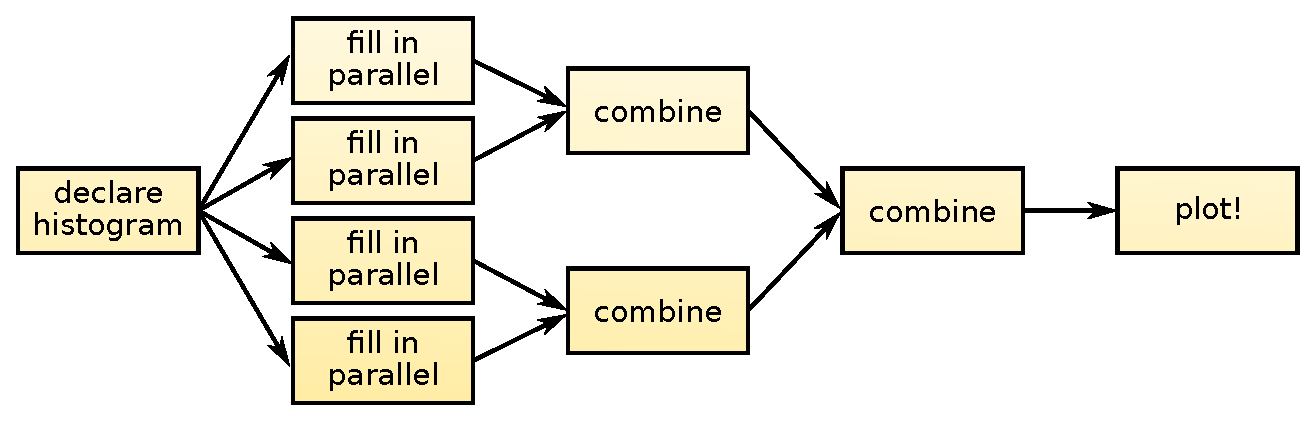
\includegraphics[width=\linewidth]{parallelization.pdf}

\vspace{-1 cm}
\[ \underbrace{\mbox{\hspace{1.5 cm}}}_{\mbox{client}} \hspace{0.25 cm} \underbrace{\mbox{\hspace{6.5 cm}}}_{\mbox{workers}} \hspace{0.5 cm} \underbrace{\mbox{\hspace{1.5 cm}}}_{\mbox{client}} \]

\end{frame}

\begin{frame}{Motivated by a different problem}

\begin{block}{Histogramming in Julia}
\end{block}

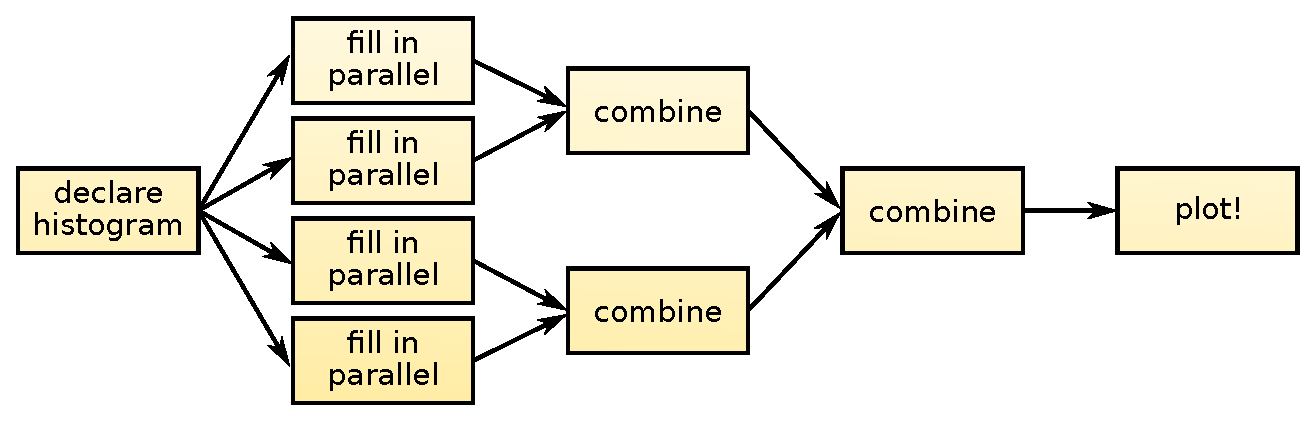
\includegraphics[width=\linewidth]{parallelization.pdf}

\vspace{-1 cm}
\[ \underbrace{\mbox{\hspace{1.5 cm}}}_{\mbox{interactive}} \hspace{0.25 cm} \underbrace{\mbox{\hspace{6.5 cm}}}_{\mbox{spawned processes}} \hspace{0.5 cm} \underbrace{\mbox{\hspace{1.5 cm}}}_{\mbox{interactive}} \]

\end{frame}

%%  HERE  %%



\begin{frame}[fragile]{Motivated by a different problem}
\begin{description}
\item[Problem:] Spark has a functional interface; ROOT's imperative TH1 classes are awkward in that paradigm.
\end{description}

\begin{columns}
\column{0.5\linewidth}
\begin{lstlisting}{language=python}
x = ROOT.TH1F("x", "", 100, 0.0, 20.0)

for event in events:
    px.fill(event.met.px)

x.Draw()
\end{lstlisting}

\column{0.5\linewidth}
\begin{lstlisting}{language=python}
x = events.aggregate(
    ROOT.TH1F("x", "", 100, -5.0, 5.0),
    lambda h, event:
      h[0].fill(event.met.px),
    lambda h1, h2:
      h1[0].Add(h2[0]))

x.Draw()
\end{lstlisting}
\end{columns}
\end{frame}

\begin{frame}[fragile]{Motivated by a different problem}
\begin{description}
\item[Problem:] Spark has a functional interface; ROOT's imperative TH1 classes are awkward in that paradigm.
\end{description}

\begin{columns}
\column{0.5\linewidth}
\begin{lstlisting}{language=python}
x = ROOT.TH1F("x", "", 100, 0.0, 20.0)
y = ROOT.TH1F("y", "", 100, 0.0, 20.0)

for event in events:
    px.fill(event.met.px)
    py.fill(event.met.py)

x.Draw()
y.Draw()
\end{lstlisting}

\column{0.5\linewidth}
\begin{lstlisting}{language=python}
x, y, z = events.aggregate(
    (ROOT.TH1F("x", "", 100, -5.0, 5.0),
     ROOT.TH1F("y", "", 100, -5.0, 5.0)),
    lambda h, event: (
      h[0].fill(event.met.px),
      h[1].fill(event.met.py)),
    lambda h1, h2: (
      h1[0].Add(h2[0]),
      h1[1].Add(h2[1])))

x.Draw()
y.Draw()
\end{lstlisting}
\end{columns}
\end{frame}

\begin{frame}[fragile]{Motivated by a different problem}
\begin{description}
\item[Problem:] Spark has a functional interface; ROOT's imperative TH1 classes are awkward in that paradigm.
\end{description}

\begin{columns}
\column{0.5\linewidth}
\begin{lstlisting}{language=python}
x = ROOT.TH1F("x", "", 100, 0.0, 20.0)
y = ROOT.TH1F("y", "", 100, 0.0, 20.0)
z = ROOT.TH1F("z", "", 100, 0.0, 20.0)

for event in events:
    px.fill(event.met.px)
    py.fill(event.met.py)
    pz.fill(event.met.pz)

x.Draw()
y.Draw()
z.Draw()
\end{lstlisting}

\column{0.5\linewidth}
\begin{lstlisting}{language=python}
x, y, z = events.aggregate(
    (ROOT.TH1F("x", "", 100, -5.0, 5.0),
     ROOT.TH1F("y", "", 100, -5.0, 5.0),
     ROOT.TH1F("z", "", 100, -5.0, 5.0)),
    lambda h, event: (
      h[0].fill(event.met.px),
      h[1].fill(event.met.py),
      h[2].fill(event.met.py)),
    lambda h1, h2: (
      h1[0].Add(h2[0]),
      h1[1].Add(h2[1]),
      h1[2].Add(h2[2])))

x.Draw()
y.Draw()
z.Draw()
\end{lstlisting}
\end{columns}
\end{frame}

\begin{frame}[fragile]{Motivated by a different problem}
\begin{columns}
\column{0.5\linewidth}
The problem is that 


\column{0.5\linewidth}
\begin{lstlisting}{language=python}
x, y, z = events.aggregate(
    # book
    (ROOT.TH1F("x", "", 100, -5.0, 5.0),
     ROOT.TH1F("y", "", 100, -5.0, 5.0),
     ROOT.TH1F("z", "", 100, -5.0, 5.0)),
    # increment
    lambda h, event: (
      h[0].fill(event.met.px),
      h[1].fill(event.met.py),
      h[2].fill(event.met.py)),
    # combine
    lambda h1, h2: (
      h1[0].Add(h2[0]),
      h1[1].Add(h2[1]),
      h1[2].Add(h2[2])))

x.Draw()
y.Draw()
z.Draw()
\end{lstlisting}
\end{columns}
\end{frame}



\end{document}
